

\chapter{Discrete Time Fourier Transform}


\section{Relation between DTFT and impulse sampled CTFT}


\begin{equation}
\begin{array}{rcl}
\omega_c \left(\text{rad/sec}\right) \, &=& \, \omega_d \, \times \, F_s \\ \\
&=& \, \displaystyle\frac{\omega_d}{T_s} 
\end{array}
\end{equation}




%*****************************************************
%*****************************************************
%*****************************************************


\chapter{The Discrete Fourier Transform}

\section{Introduction}

The discrete Fourier transform is a \tbi{numerical technique} which computes the DTFT (discrete time Fourier transform) and CTFT (continuous time Fourier transform). In other words, there is \tbi{no transformation from time to frequency domain}.


\section{Formula and Direct Results}

\underline{Goal:} Compute Numerically DTFT and CTFT. We start by DTFT.\\

\underline{Note:} To see the derivation, review the slides.


\subsection{Discrete time case: DFT of DTFT}

Let $f[k]$ a discrete signal with index $k$, of length $N_0$.


\begin{equation}
\begin{array}{rcl}
\text{DFT}\{f[k]\} \, &=&\, F_r \\
						&=& \, F(r \, \Omega_0) \\
					   &=&\, \displaystyle\sum_{k \, = \, 0}^{N_0 \, - \, 1} \, f[k] \, \text{exp} \left(\, -j r \Omega_0 \, k   \,\right)
\end{array}
\label{Eq:DFT:dft_for_dtft}
\end{equation}
 
where $\begin{cases}
r \, = \, 0,1,2, \rightarrow \, N_0 \, - \, 1 \\
\Omega_0 \, = \,  \displaystyle\frac{2 \, \pi}{N_0} \, = \, \text{freqeuncy step at which we sample the DTFT spectrum}
\end{cases}$\\


\underline{Inverse DFT case:}\\

\begin{equation}
\begin{array}{rcl}
f[k] \, &=&\, \displaystyle\frac{1}{N_0} \, \displaystyle\sum_{r \, = \, 0}^{N_0 \, - \, 1} \, F_r \, \text{exp} \left(\, -j r \Omega_0 \, k   \,\right)
\end{array}
\end{equation}

\newpage
\subsection{Continuous time case: DFT of CTFT}

\begin{itemize}

\item Let $f(t)$ be a continuous time signal of duration $\tau$.

\item Sample the signal $f(t)$ over a period $T_0 \, \leq \, \tau$, where $T_s$ is the sampling time. 

	\begin{itemize}
	\item The \tbi{number of sample} we get is $N_0 \, = \, \displaystyle\frac{T_0}{T_s} \, = \, T_0 \, \times \, F_s$
	\end{itemize}

\item Formula:

\begin{equation}
\begin{array}{rcl}
\text{DFT}\{f[t]\} \, &=&\, F_r \\
						&=& \, F(r \, \omega_0) \\
					   &=&\, \displaystyle\sum_{k \, = \, 0}^{N_0 \, - \, 1} \, f_k \, \text{exp} \left(\, -j r \Omega_0 \, k   \,\right)
\end{array}
\end{equation}

where $\begin{cases}

\omega_0 \, = \, 2 \, \pi \, F_0 \, \text{rad/s} \, (\text{from spectral sampling theorem}) \\
\Omega_0 \, = \, \omega_0 \, T_s \, = \,   \displaystyle\frac{2 \, \pi}{N_0} \, = \, \text{sampling interval at wihich we sample the spectrum of the CTFT} \\
f_k \, = \, T_s \, f(k \, T_s)
\end{cases}$ 



\end{itemize}


\section{Examples}

\subsection{Continuous time case: Infinite Time}
\label{Sub:DFT:Continuous_time_Infinite_Time}

The signal is: $x(t) \, = \, \text{exp}(-0.5 \, t) \, u(t) \leftrightarrow \, X(\omega) \, = \, \displaystyle\frac{1}{j \, \omega\, + \, 0.5}$.\\

The Fourier transform can be found by any look up table.


\begin{figure}[h]
\centering
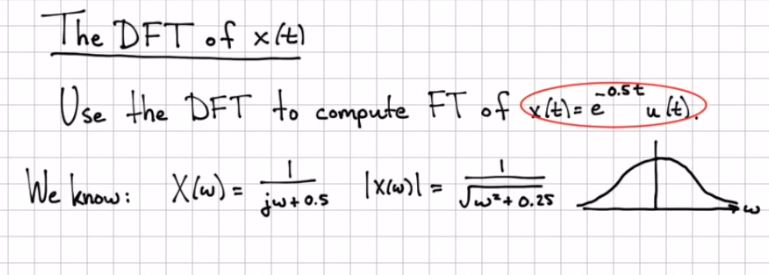
\includegraphics[width = 0.7\textwidth, frame]{Figures/DFT/example_cont_time}
\caption{Given: Infinite time and infinite frequency signal}
\label{fig:DFT:example_cont_time}
\end{figure}


\begin{itemize}

\item To compute the DFT, we need to sample in the time domain ($f_k$) , and take samples in the frequency domain ($\Omega_0$).

\item However $x(t)$ in infinite in time and hence infinite in frequency, and there is no max frequency to apply the sampling period to.

	\begin{itemize}
	\item Need to do some engineering judgment about this.
	\end{itemize}

\item We can put the following criteria: what is the value of $\omega$ at which the frequency content is bellow 2 \% ?

	\begin{itemize}
	\item So we capture 98 \% of the frequency content of the signal
	
	\item This value of $\omega \, = \, 50 \text{rad/s} \leftrightarrow \, B \, = \,  \displaystyle\frac{25}{\pi}$ Hz as shown in \autoref{fig:DFT:capture_sampling_period}
	
\begin{figure}[h]
\centering
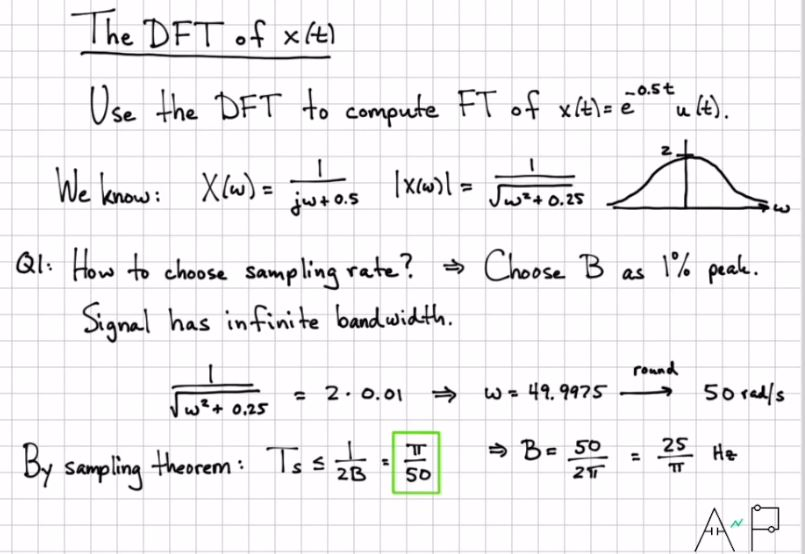
\includegraphics[width = 0.7\textwidth, frame]{Figures/DFT/capture_sampling_period}
\caption{Solving for the sampling period $T_s$}
\label{fig:DFT:capture_sampling_period}
\end{figure}

	\item The we solve for the $T_s$ and we get that we need to sample at a rate $\displaystyle\frac{\pi}{50}$ seconds (this the minimum, we could sample faster, we see the effect of this later) 
	
	\end{itemize}

\item After we solve for $T_s \, = \, \displaystyle\frac{\pi}{50}$ s, there is another question to be asked: for \tbi{how long do we need to sample}?

	\begin{itemize}
	\item This signal is going forever, we can't just keep sampling forever
	\end{itemize}

\item So we need to solve for $T_0$

\newpage
\item We know that the signal is a decaying exponential, we can see for some value of $T_0$ where the amplitude value of $x(t)$ are very low, and by this we are not throwing some high value amplitude (information)

\item Computation shown in \autoref{fig:DFT:when_stop_sample}.

\begin{figure}[h]
\centering
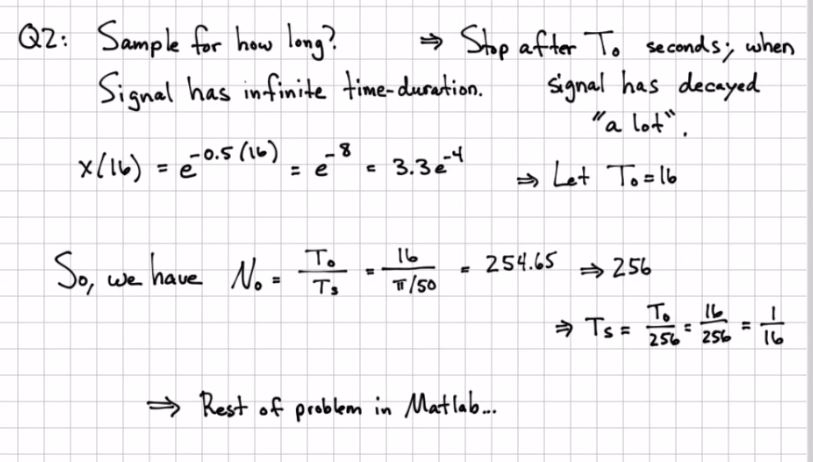
\includegraphics[width = 0.7\textwidth, frame]{Figures/DFT/when_stop_sample}
\caption{Solving for the sampling period $T_s$}
\label{fig:DFT:when_stop_sample}
\end{figure}

	\begin{itemize}
	\item We try for example for $T_0 \, = \, 16$s, we get $x(16) \, = \, 3.3 \, e^-4$, very small number
	
	\item If we choose $T_0 \, = \, 16$, the number of sample we get in this period using a sampling rate $T_s \, = \, \displaystyle\frac{\pi}{50}$ is: $N_0 \, = \, \displaystyle\frac{T_0}{T_s} \, = \, 254.65$
	
	
	\item However, the number of samples we need to grab need to be integer, so let's say we need to grab 256 samples
	
	\item We resolve again for $T_s$ using $N_0 \, = \, 256$ samples, and we get $T_s \, = \, \displaystyle\frac{1}{16}$ seconds
	
	\end{itemize}

\end{itemize}


The rest of the problem is done via coding.


As a summary we have:

\begin{itemize}

\item First question we ask since the signal $x(t)$ isn't band limited in the frequency domain: how do we choose the sampling rate $T_s$

	\begin{itemize}
	\item $T_s \, = \, \displaystyle\frac{1}{16}$ seconds
	\end{itemize}
	
\item $\mathrm{2}^\mathrm{nd}$ question: for how long we keep sampling ?

	\begin{itemize}
	\item $T_0 \, = \, 16$ s, which give $N_0 \, = \, 256$ samples/second
	such that $T_s \, = \, \displaystyle\frac{1}{16}$ s
	\end{itemize}

\end{itemize}


\underline{Some Tuning and Analysis:}\\

2 factors influence the results of the DFT values: the sampling period $T_s$ and signal duration $T_0$, which specify for how long we keep doing sampling. Let's try to change each factor while fixing the other.\\

\underline{Changing signal duration $T_0$:}\\


The results of the computation are shown in \autoref{fig:DFT:cont_time_signal_duration}.

\begin{itemize}

\item The base line is the first row where $F_s \, = \, 16 \text{ sample}/\,\text{s}$ and $T_0 \, = \, 16$s, as in the theoretical part

\item First we truncate (throw away) the signal allot, which means $T_0$ decrease (decrease to 2 s in our choice)

	\begin{itemize}
	\item Since $\Omega_0 \, = \, \displaystyle\frac{2 \, \pi}{N_0}$ and $N_0 \, = \, \displaystyle\frac{T_0}{T_s}$, so we get less number of coefficient for DFT computation
	
	\item And notice that the values of the DFT in the $\mathrm{2}^\mathrm{nd}$ plot are below the blue curve
	\end{itemize}	 

\item When we increase the signal duration (truncate less) things tend to be better.

\end{itemize}

As a conclusion, even if the sampling rate $F_s$ is good enough but we truncate the signal allot in the time domain, the spectral representation will not be good and we loss frequency content of the signal.

\begin{figure}[h]
\centering
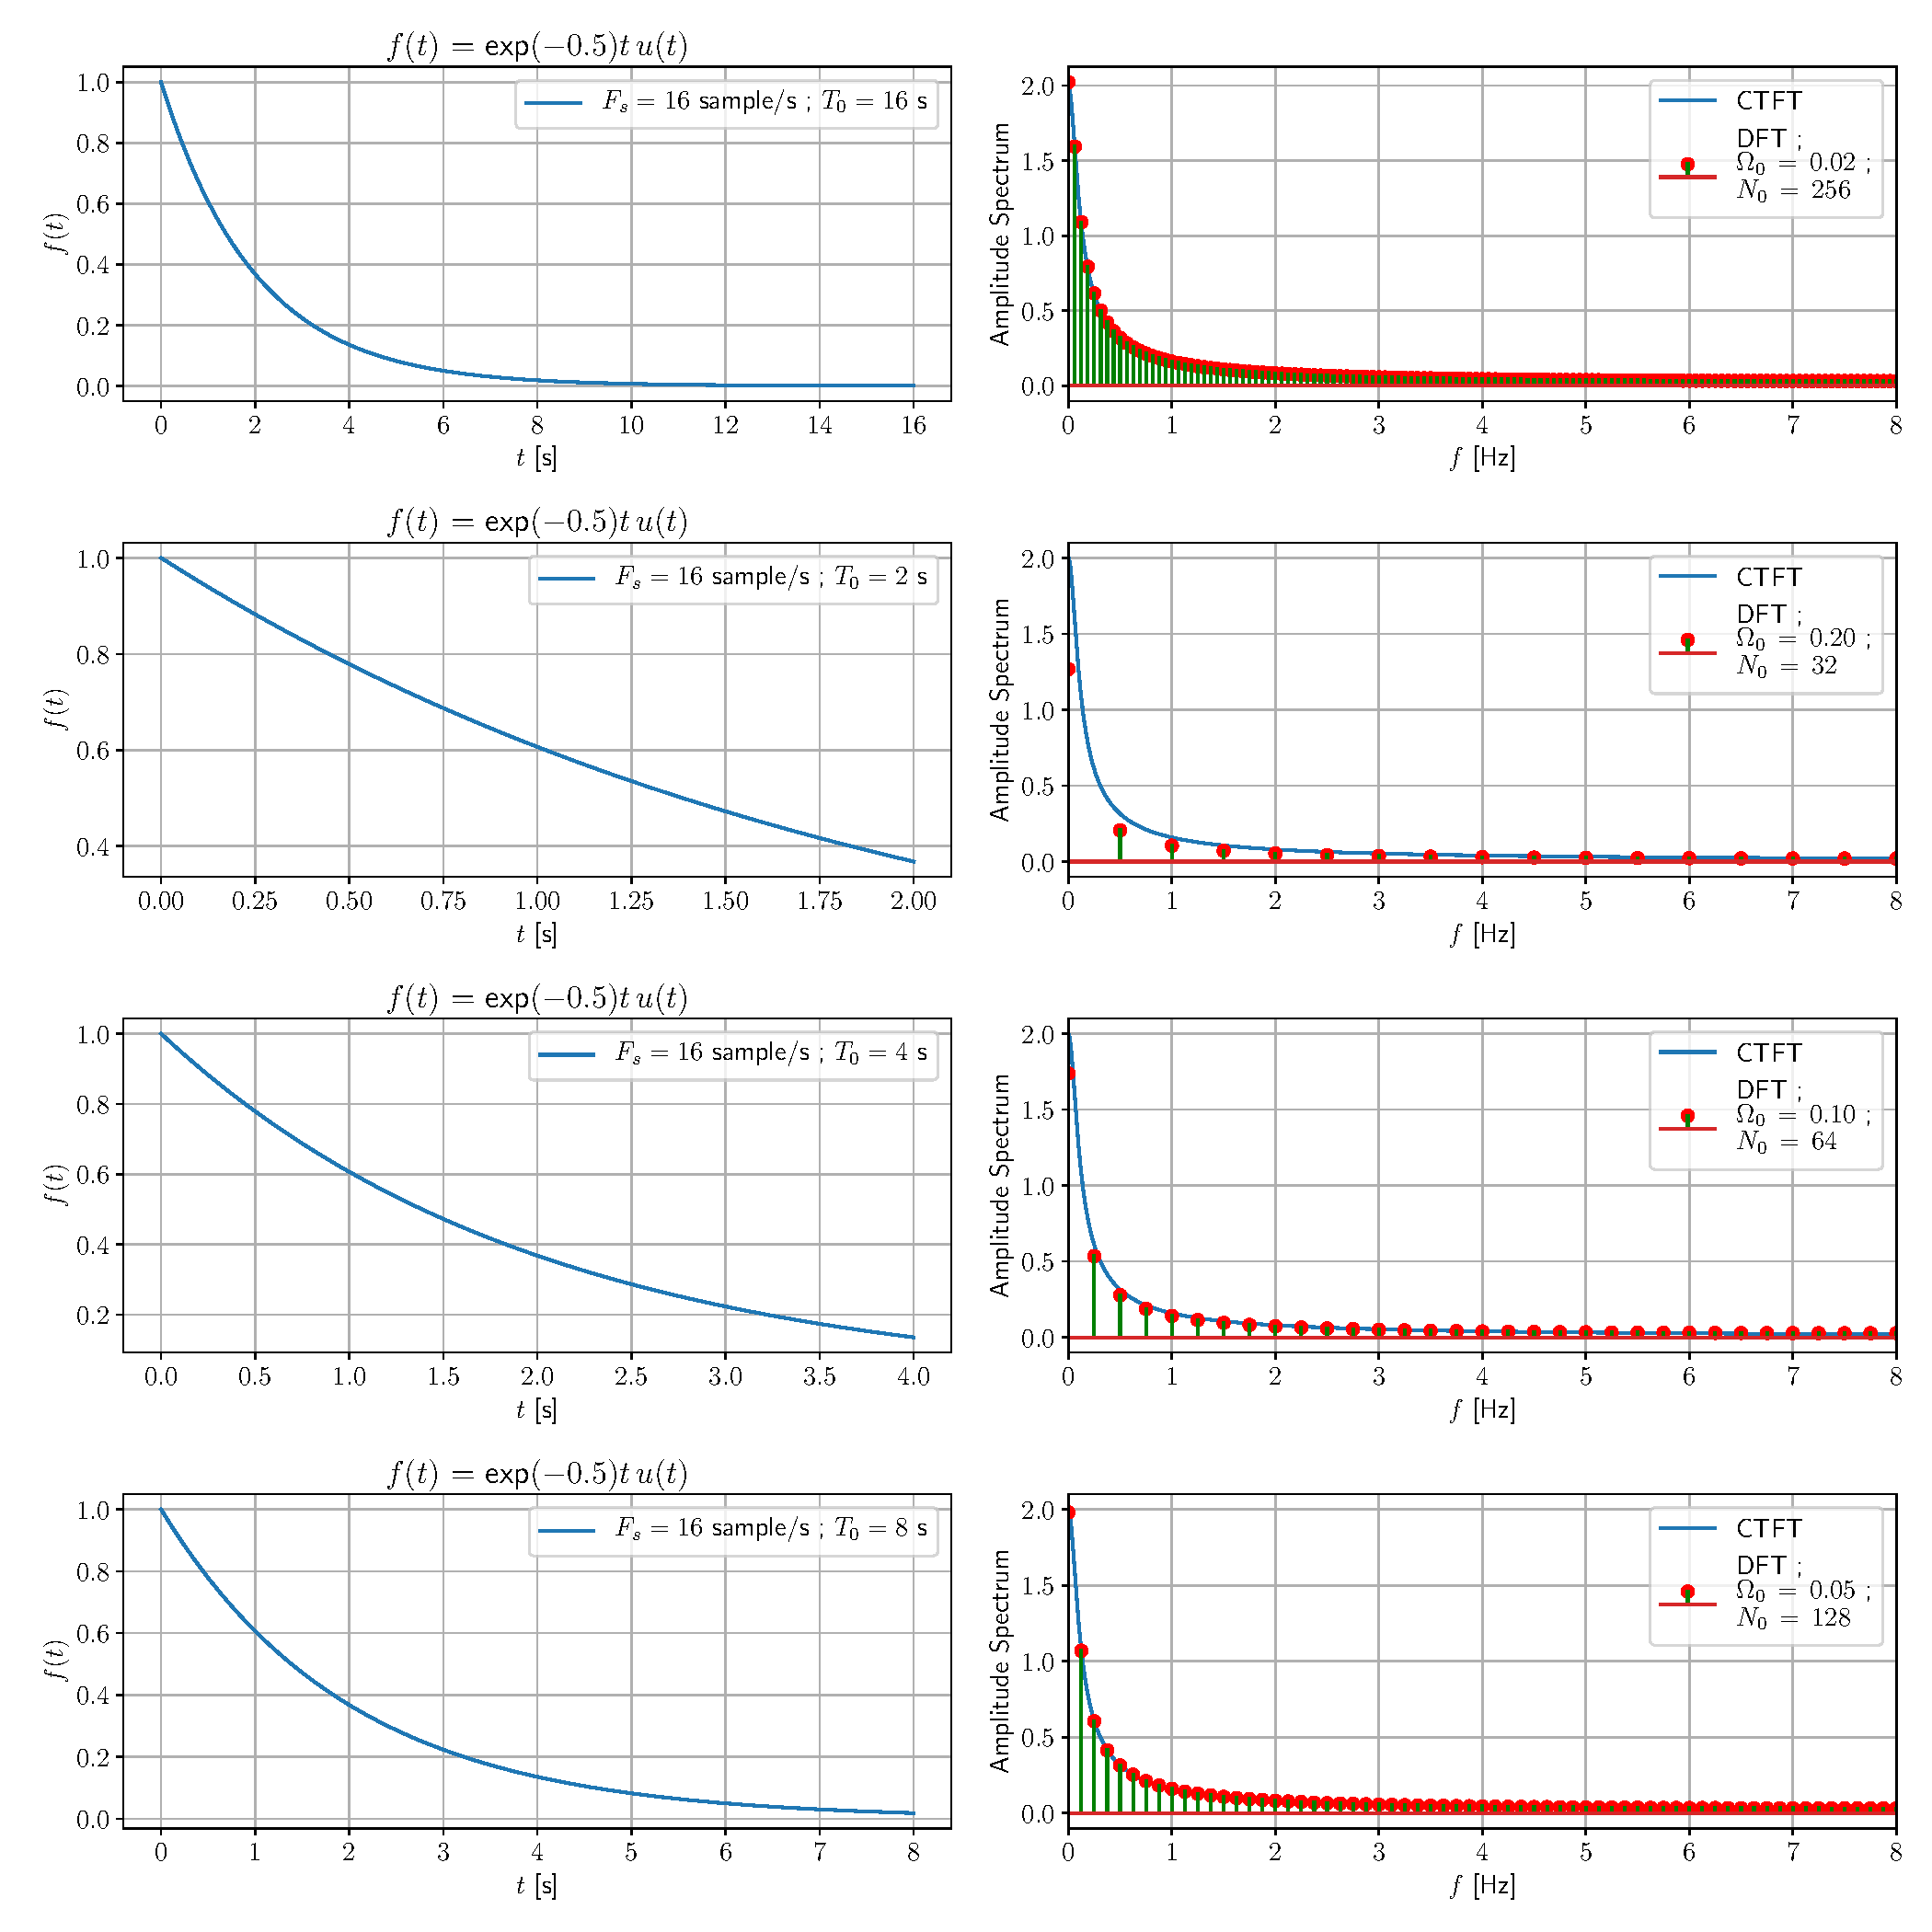
\includegraphics[width = 0.7\textwidth, frame]{Figures/DFT/DFT_Continous_time_signal_duration}
\caption{DFT results for example of \autoref{fig:DFT:example_cont_time}: Signal Duration $T_0$ and its effect on DFT}
\label{fig:DFT:cont_time_signal_duration}
\end{figure}

\newpage
\underline{Changing the sampling rate $F_s$:}\\

Results are shown in \autoref{fig:DFT:cont_time_sampling_rate}.

\begin{figure}[h]
\centering
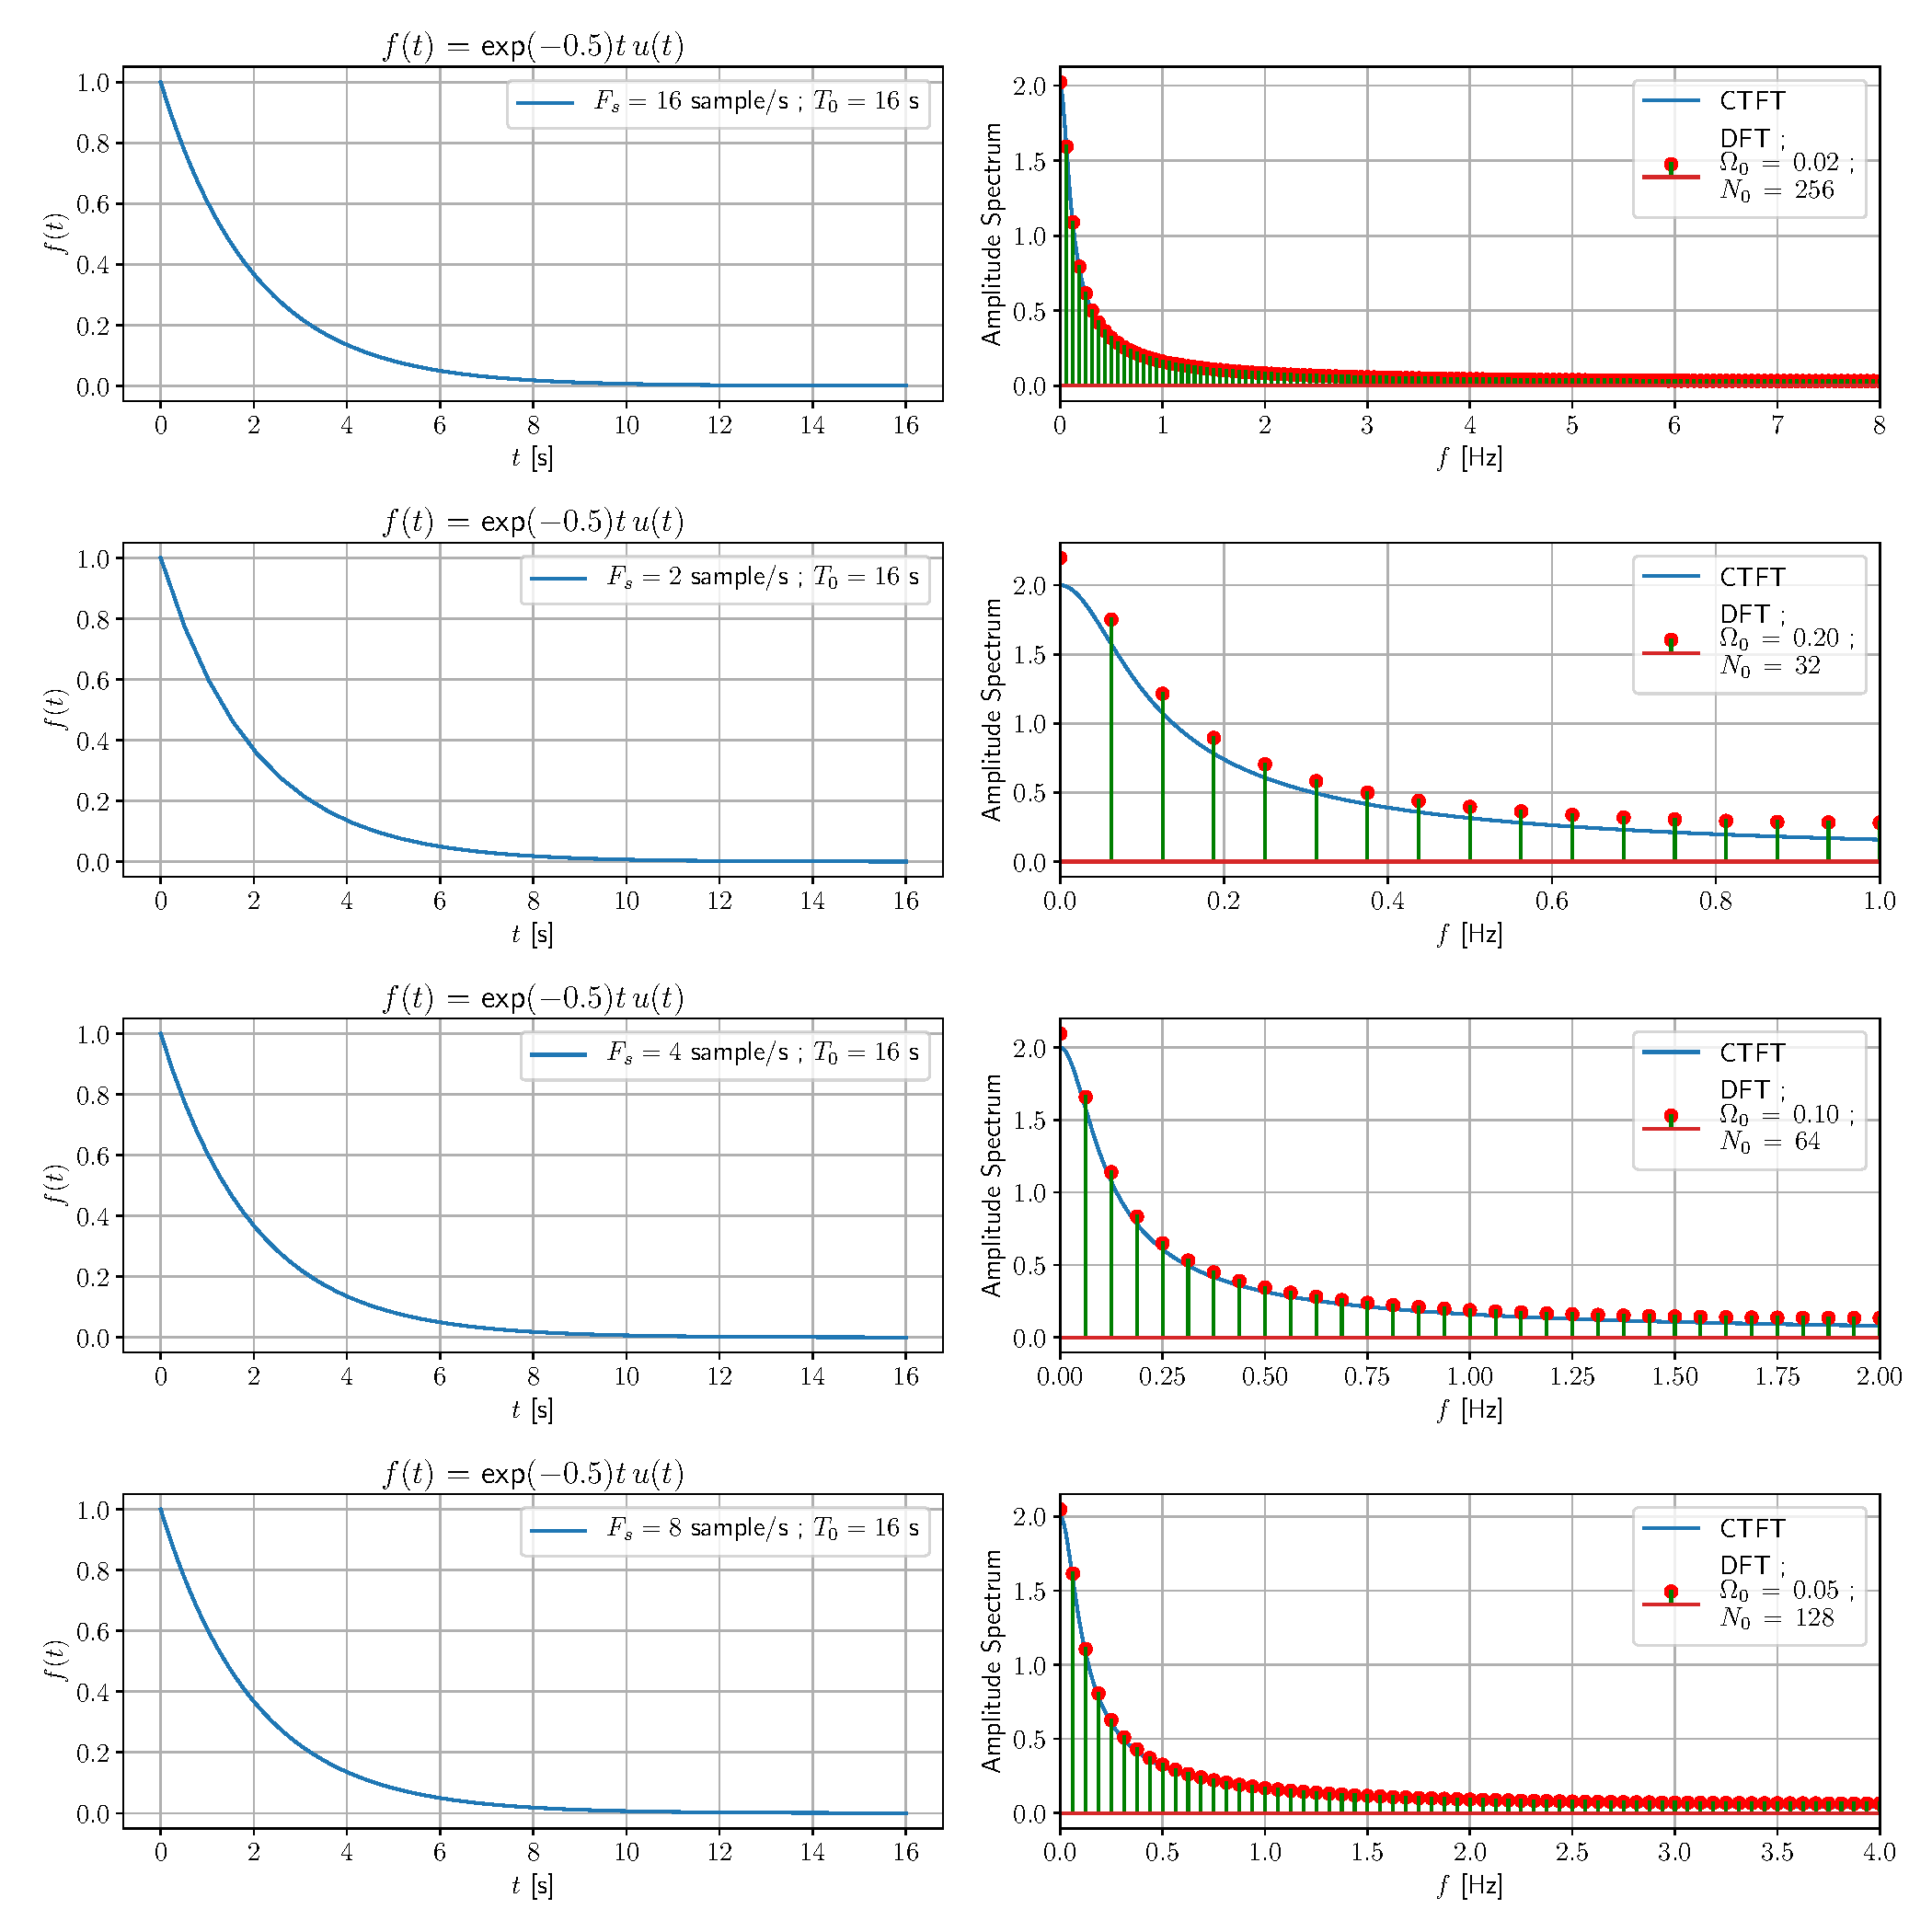
\includegraphics[width = 0.7\textwidth, frame]{Figures/DFT/DFT_Continous_time_sampling_rate}
\caption{DFT results for example of \autoref{fig:DFT:example_cont_time}: Sampling rate $F_s$ and its effect on DFT}
\label{fig:DFT:cont_time_sampling_rate}
\end{figure}

\begin{itemize}

\item As usual the first plot is the base line: $F_s \, = \, 16 \text{ sample/s}$ and $T_0 \, = \, 16$s.

\item Notice that for example when $F_s \, = \, 2 \text{ sample/s}$ (8 times less than the true one), the DFT values are above the true curve of the CTFT.

\end{itemize}



\newpage
\subsection{Discrete Time: Finite Length Signal}

The problem is shown in \autoref{fig:DFT:discrete_case_finite_length}.

\begin{figure}[h]
\centering
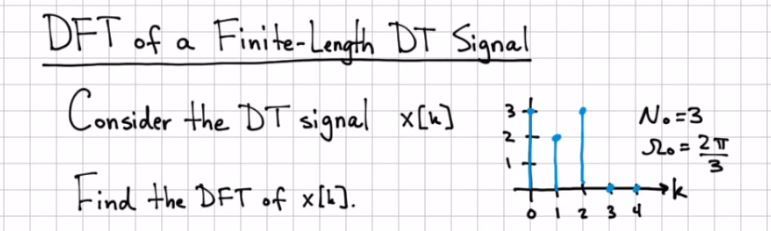
\includegraphics[width = 0.7\textwidth, frame]{Figures/DFT/discrete_case_finite_length}
\caption{Discrete time signal: finite length}
\label{fig:DFT:discrete_case_finite_length}
\end{figure}

\begin{itemize}

\item It has 3 non-zero values at indices 0,1 and 2, so $N_0 \, = \, 3$

\item Since $N_0 \, = \, 3$, so the DFT components for the DTFT will be also 3: $r: 0 \, \rightarrow \, 2$

\item The \tbi{sampling interval} at which we compute the DFT coefficient values is $\Omega_0 \, = \, \displaystyle\frac{2\, \pi}{N_0} \, = \, \displaystyle\frac{2\, \pi}{3}$

	\begin{itemize}
	\item So we compute the value at $0 \, \Omega_0 \, , 1 \, \Omega_0\,$ and $2 \, \Omega_0 $
	\end{itemize}

\end{itemize}


Since the values of the DFT are only 3, we can do the computation by hand easily using equation (\ref{Eq:DFT:dft_for_dtft}). The computations are shown in \autoref{fig:DFT:discrete_case_finite_length_computation} 


\begin{figure}[h]
\centering
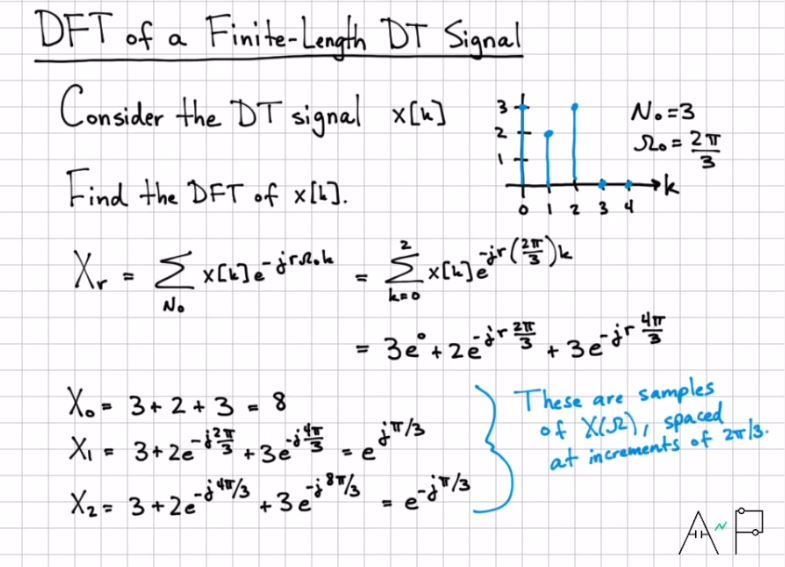
\includegraphics[width = 0.7\textwidth, frame]{Figures/DFT/discrete_case_finite_length_computation}
\caption{Computing DFT values of the DTFT using equation (\ref{Eq:DFT:dft_for_dtft})}
\label{fig:DFT:discrete_case_finite_length_computation}
\end{figure}

	\begin{itemize}
	\item First we compute a formula as a function of $r$ for all values of time index $k$
	
	\item Then we plug each value of $r$ to obtain $X_0 \, , \, X_1$ and $X_2$
	\end{itemize}

\newpage
Now to compare the result of the DFT values, we compute also the expression of DTFT, detailed in \autoref{fig:DFT:dtft_expression}.

\begin{figure}[h]
\centering
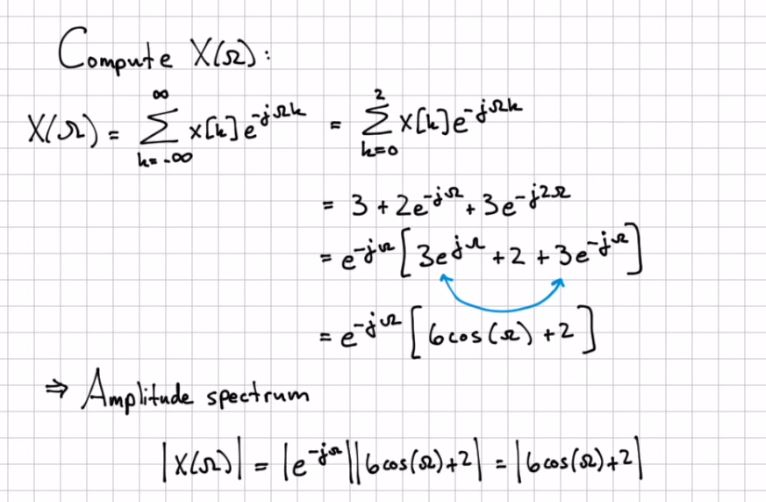
\includegraphics[width = 0.7\textwidth, frame]{Figures/DFT/dtft_expression}
\caption{Computing DTFT expression for comparison with DFT values}
\label{fig:DFT:dtft_expression}
\end{figure}

\newpage
\underline{Results and Analysis:}\\

Results are shown in \autoref{fig:DFT:discrete_case_finite_length_results}.

\begin{figure}[h]
\centering
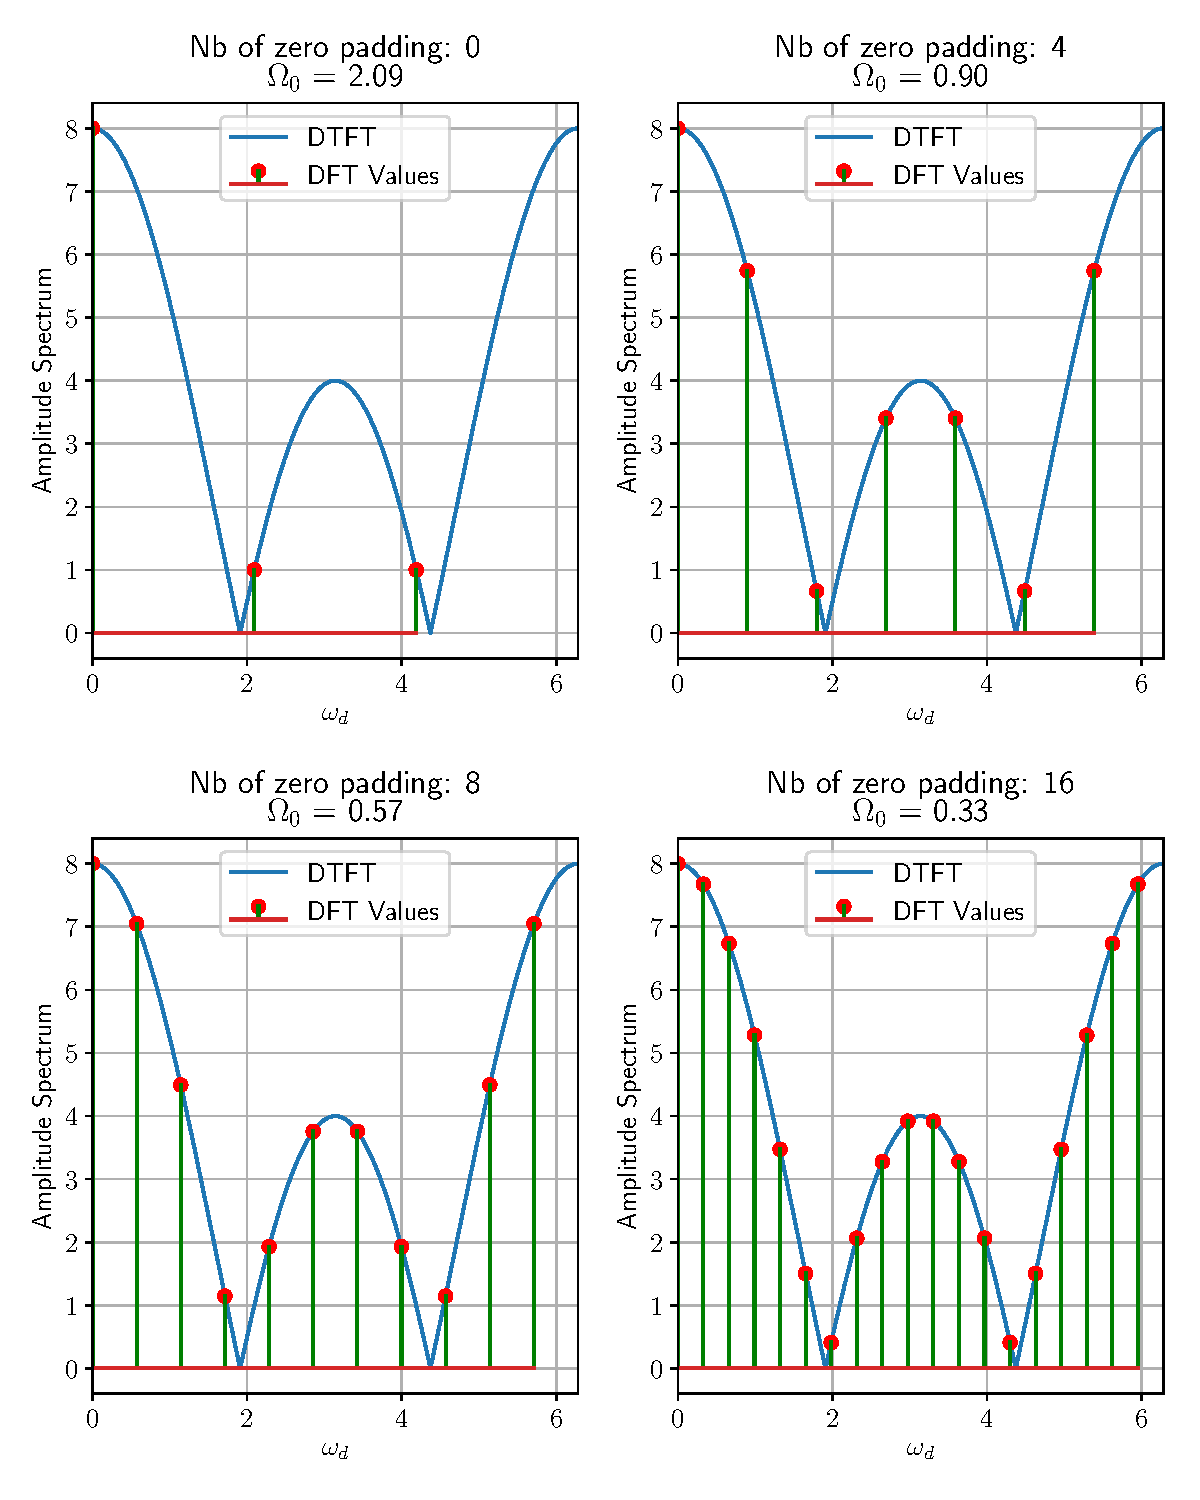
\includegraphics[width = 0.7\textwidth, frame]{Figures/DFT/DFT_Discrete_time_Finite_Length}
\caption{Results of Example of  \autoref{fig:DFT:discrete_case_finite_length} \\ $ 0 \, \leq \,  \omega_d \leq \, 2 \, \pi$}
\label{fig:DFT:discrete_case_finite_length_results}
\end{figure}

\begin{itemize}

\item The result are also made with respect to \tbi{zero padding} effect

	\begin{itemize}
	\item We pad (add) zeros values to the signal in the time (discrete) domain
	
	\item This won't affect the signal, only the number of samples will increase
	
	\end{itemize}

	\item Recall that the sampling interval $\Omega_0 \, = \, \displaystyle\frac{2\, \pi}{N_0}$ where $N_0$ is the length of the signal
	
	\item If we add more samples $N_0$, $\Omega_0$ will decrease and hence we take more samples of the spectrum of the DTFT.

\end{itemize}

\newpage
\subsection{Discrete Time: Infinite Length Signal}

Now we move with infinite length discrete time signal. As in \ref{Sub:DFT:Continuous_time_Infinite_Time}, since we are dealing with infinite length sequence, we need to truncate the signal in the time (discrete) domain and make the index sampling $k$ between 0 and $N_0 \, - 1$. Given are shown in \autoref{fig:DFT:discrete_case_Infinite_length_given}

\begin{figure}[h]
\centering
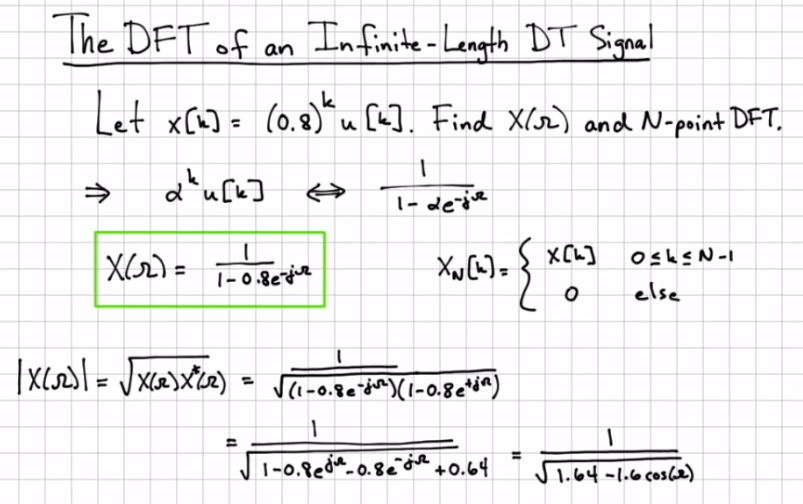
\includegraphics[width = 0.7\textwidth, frame]{Figures/DFT/DFT_Discrete_time_Infinite_Length_given}
\caption{DFT for infinite length discrete time signal}
\label{fig:DFT:discrete_case_Infinite_length_given}
\end{figure}

Results are shown in \autoref{fig:DFT:discrete_case_Infinite_length_results}.

\begin{itemize}

\item $k$ is the sampling index in the discrete time domain

\item The base $a \, = \, 0.8$ in all cases

\item $p$ is the number of samples we get:

	\begin{itemize}
	\item The more $p$ we get, the \tbi{less we truncate the signal in the discrete time domain}, and hence the DTFT using the loop formula and the DFT values will get more accurate to analytical DTFT formula
	\end{itemize}

\end{itemize}
 
\newpage
\begin{figure}[h]
\centering
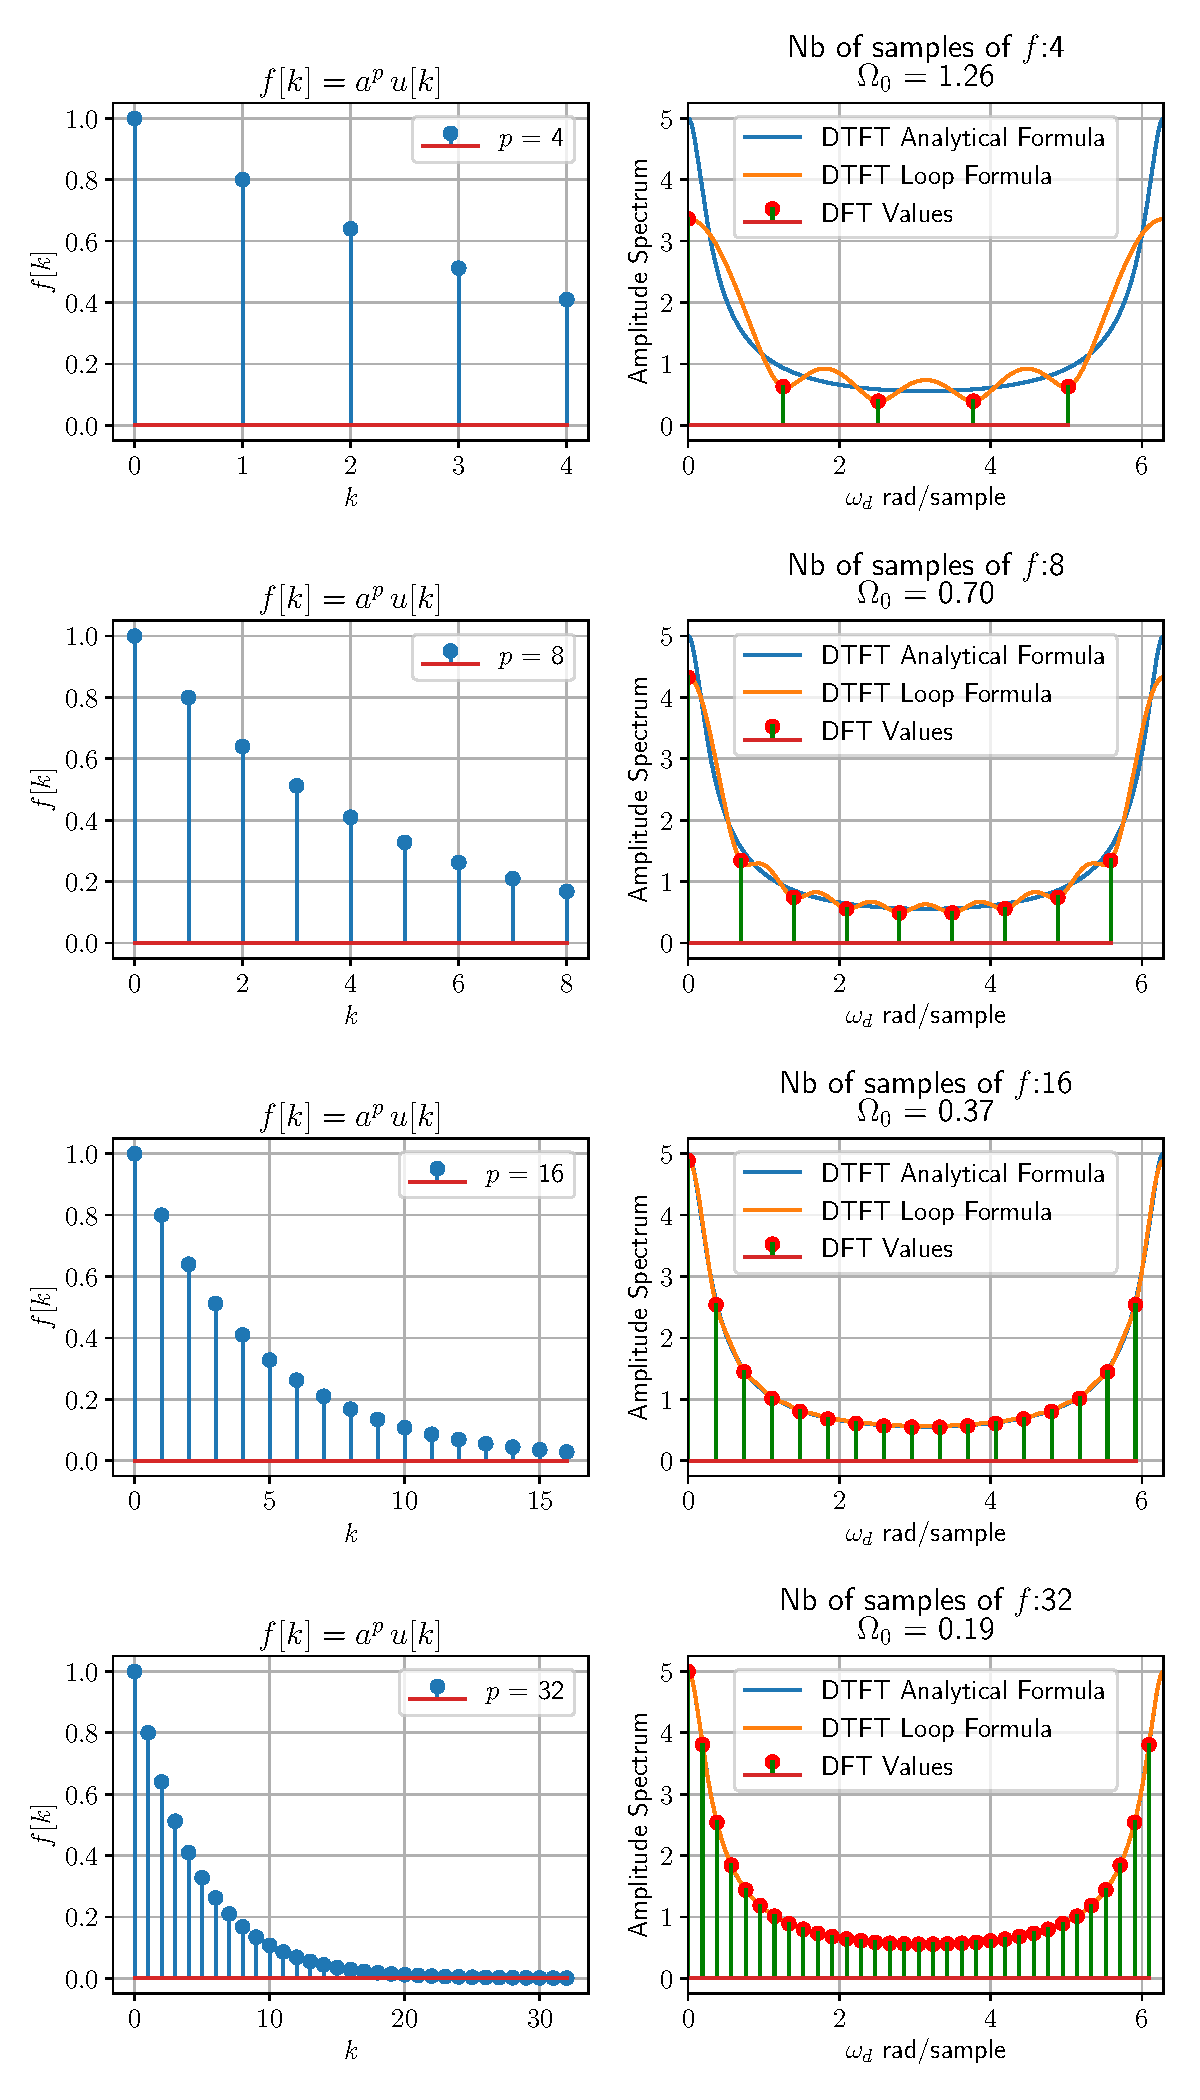
\includegraphics[width = 0.6\textwidth, frame]{Figures/DFT/DFT_Discrete_time_Infinite_Length}
\caption{Result of example of \autoref{fig:DFT:discrete_case_Infinite_length_given}}
\label{fig:DFT:discrete_case_Infinite_length_results}
\end{figure} 




\newpage

\section{Resolution and Zero Padding}

After taking all possible cases of DFT computations for continuous and discrete time signals, we do some analysis of frequency resolution using 2 sin function.

\begin{figure}[h]
\centering
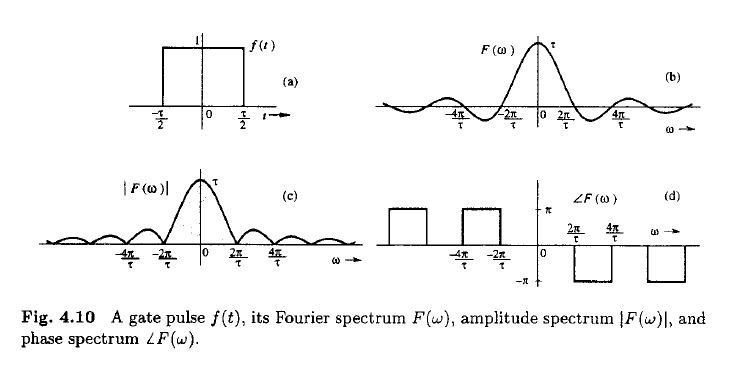
\includegraphics[width = 0.7\textwidth, frame]{Figures/DFT/rect_Fourier_transform}
\caption{rect Fourier Transform}
\label{fig:DFT:rect_Fourier_transform}
\end{figure} 

\begin{itemize}

\item Recall that $\text{sin}(\omega_0 \, t) \leftrightarrow \, j\,\pi \, \left[\, \delta(\omega_c \,- \, \omega_0) \, + \, \delta(\omega_c \,+ \, \omega_0)  \,\right]$

\item When we compute the Fourier transform of $\text{sin}(\omega_0)\, t$, the signal in theory has domain  $-\infty < \, t \, <\, + \infty$, but in reality we need to truncate the signal (or cut it), so we multiply it by a rect (pulse)

	\begin{itemize}
	\item Recall that $\text{rect} \left(\, \displaystyle\frac{t}{\tau} \,\right) \, \leftrightarrow \, \text{sinc} \left(\,\displaystyle\frac{\omega_c \, \tau}{2} \, \right)$ shown in \autoref{fig:DFT:rect_Fourier_transform}.

	\end{itemize}

\end{itemize}

Important Note about Data truncation:

\begin{itemize}

\item Let $f(t)$ some signal we want to study and $w(t)$ some window function we use where $\begin{cases}
f(t) \leftrightarrow F(\omega_c) \\
w(t) \leftrightarrow W(\omega_c) 
\end{cases}$

\item Truncation is done by multiplying the function by some window. Mathematically: 


\begin{equation}
f_w(t) \, = \, f(t) \, \times \, w(t) \leftrightarrow \, F_w(\omega_c) \, = \, F(\omega_c) \, * \, W(\omega_c)
\label{Eq:DFT:windowing_1} 
\end{equation}

	\begin{itemize}
	
	\item $f_w(t)$ denote the window signal resulting from windowing the original signal $f(t)$
	
	\item Multiplication in the time domain result in convolution in the frequency domain
	
	\item By the convolution width property, the width of the resulting signal will be the sum of the width of the 2 signal
	
	\item So as an intuition, the bandwidth of $F(\omega_c)$ will increase by the amount of the bandwidth of window function we use $W(\omega_c)$
	\end{itemize}



\item Solving equation (\ref{Eq:DFT:windowing_1}):

\begin{equation}
\begin{array}{rcl}
F_w(\omega_c) \, &=& \, F(\omega_c) \, * \, W(\omega_c) \\ \\
				 &=& \, \left(\, j\,\pi \, \left[\, \delta(\omega_c \,- \, \omega_0) \, + \, \delta(\omega_c \,+ \, \omega_0)  \,\right]   \,\right) \, * \, \text{sinc} \left(\,\displaystyle\frac{\omega_c \, \tau}{2} \, \right) \\ \\
				&=& \, \text{sinc} \left(\,\displaystyle\frac{ \tau \, \times \, (\omega_c \, - \omega_0) }{2} \, \right) \, + \, \text{sinc} \left(\,\displaystyle\frac{ \tau \, \times \, (\omega_c \, + \omega_0) }{2} \, \right) 
\end{array}
\label{Eq:DFT:windowing_2}
\end{equation}

	\begin{itemize}
	\item We have the use the property of convolution with dirac function: when convolving a function with a dirac function, the function will be shifted to the dirac location.
	\end{itemize}

\item Equation (\ref{Eq:DFT:windowing_2}) is illustrated in \autoref{fig:DFT:window_effect}

\begin{figure}[h]
\centering
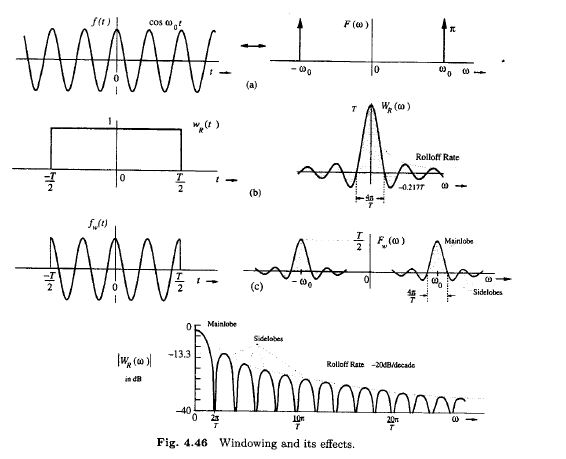
\includegraphics[width = 0.7\textwidth, frame]{Figures/DFT/window_effect}
\caption{Window effect: \tbi{spectral spreading} and \tbi{leakage}}
\label{fig:DFT:window_effect}
\end{figure} 


	\begin{itemize}
	
	
	\item The wider the window we use, the less we truncate
	
		
	\begin{itemize}
	\item Since the bandwidth of the signal is inversely proportion
	\end{itemize}
	
	
	\end{itemize}




\end{itemize}

\newpage
\subsection{1 Sinusoidal Analysis}

Consider the signal $f(t) \, = \,2 \, \text{sin} \left(\,2 \pi 500 t \,\right)$. where $F_s \, = \, 8000$ sample/s.

The study again will be by changing 2 factors: number of samples we take in the time domain (so window length) and zero padding.\\


\underline{Zero Padding Effect:}\\

We fix in this study the number of samples in the time domain (window length) and see the effect of zero padding.\\

\tbi{Rule:} zero padding doesn't effect the frequency resolution. In our case, the main lobe width will be the same whatever zero padding factor we use.

The only thing zero padding give is more sampling of the frequency spectrum, so we can get more point when plotting.

Results are shown in \autoref{fig:DFT:Spectral_Analysis_1_Sin_zero_padding}.


\begin{figure}[h]
\centering
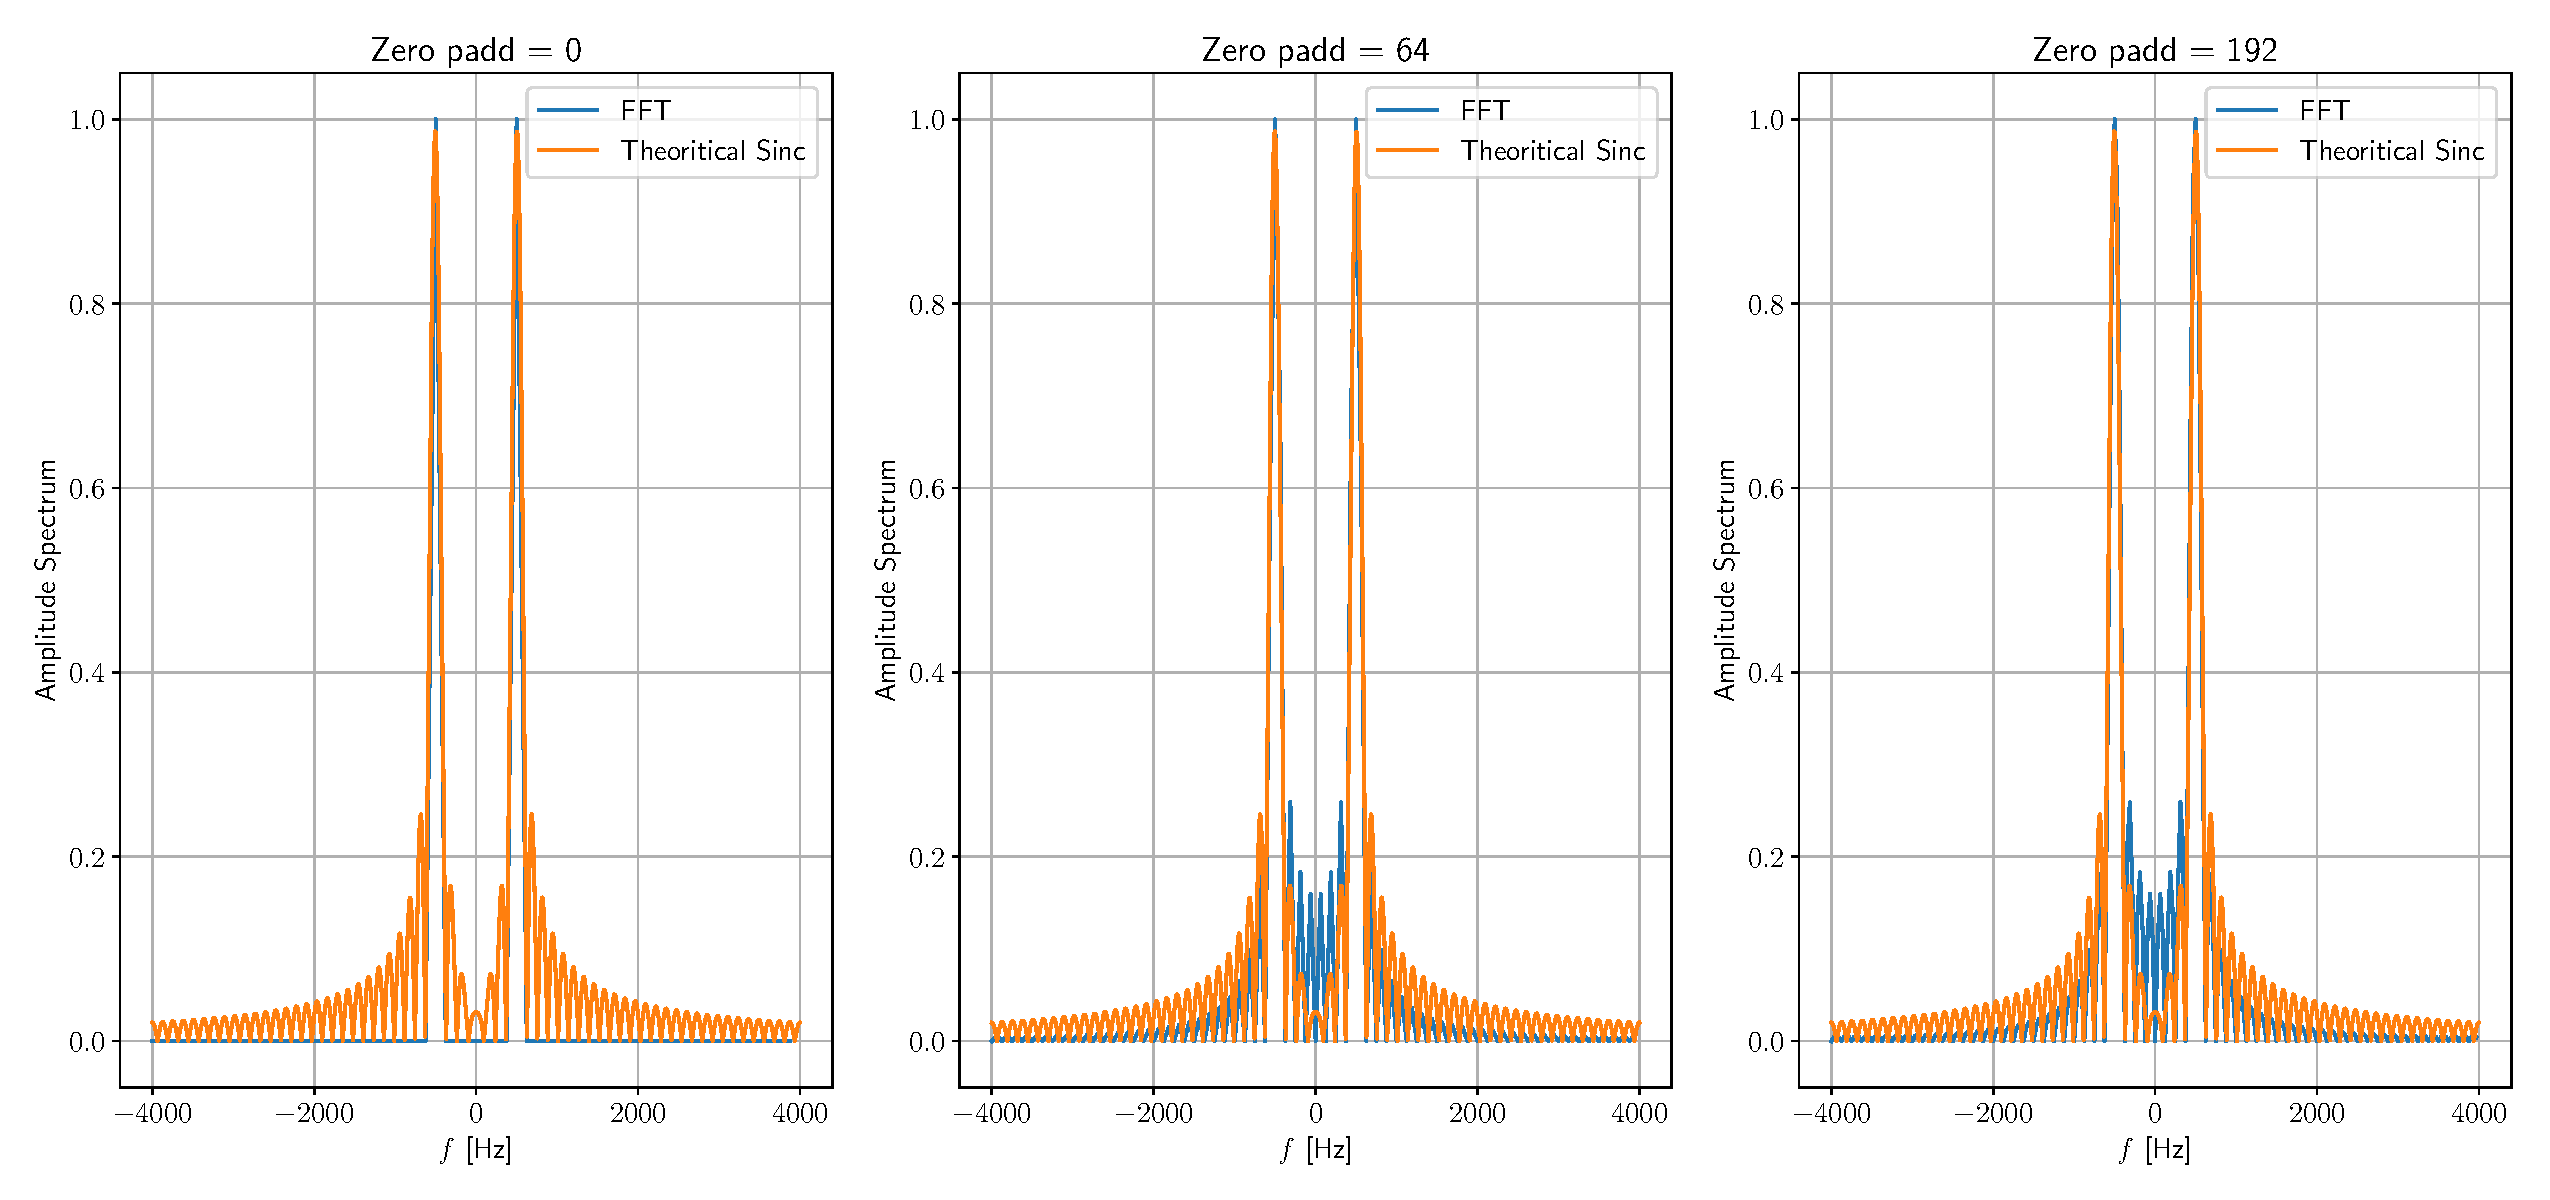
\includegraphics[width = 0.7\textwidth, frame]{Figures/DFT/Spectral_Analysis_1_Sin}
\caption{Zero Padding Effect: More samples in the frequency domain}
\label{fig:DFT:Spectral_Analysis_1_Sin_zero_padding}
\end{figure} 



%*****************************************************
%*****************************************************
%*****************************************************


\chapter{The Discrete Fourier Transform (Enhanced)}

\underline{Reference:} This way of introduction via the DTFT is from \cite{DSP_Proakis}.

\section{Introduction}

\begin{itemize}
    \item The DFT is a tool to approximate CTFT and DTFT
    
    \item First in \cite{DSP_Proakis} he talk about approximating DTFT
    
    \item Motivation for DFT:
    
        \begin{itemize}
            \item In analysing data, we always have samples and not continous time signals
            
            \item Even if we want to plug in $x[n]$ in the formula of the DTFT, we need also to evaluate on infinite grid over $[\-pi \, + \pi]$, and in computer we can't do this $\rightarrow$ this rise the need of approximation and evaluating DTFT over finite grid in $[\-pi \, + \pi]$
        \end{itemize}
    
    
    \item Be aware when using IDFT, the formula is for $N$ points, and it doesn't include zero padding option
    
        \begin{itemize}
            \item In other words, if use $M \, > \, N$ points for DFT, the IDFT use only the original $N$ points
        \end{itemize}
    
    
    \item After finishing up with the DTFT, we will see the relation between the DTFT, CTFT and DFT
    
    
    \item FFT is an algorithm to implement the DFT in an efficient manner
    
        \begin{itemize}
            \item Although people say \textit{the} FFT, but in reality there is many version of the FFT
        \end{itemize}
    
\end{itemize}


\section{Finite Duration Case}

\begin{itemize}
    \item In this section, the focus were on the understanding of the DFT for the DTFT of some finite duration signal $x[n]$
    
    
    \begin{itemize}
        \item How to take the frequency step
        
        \item How to compute the DFT Formula
        
        \item The idea of zero-padding and how it enhance the only the shape of the DFT spectrum
    \end{itemize}
    
    
\end{itemize}


\section{Infinite Duration Case}
\label{Sec:DFT:Infinite_Duration}
Now we move to the infinite duration case.

\begin{itemize}
    
\item \underline{Slide 11:}
    
        \begin{itemize}
            \item When doing this example, Prof Mark started with the case of a finite duration signal, then armed with this kind of understanding, we will tackle infinite duration case
            
            
            \item Now some person wonder: practical signal are always finite in duration, and no signal can just keep going forevever.\\
            
            Well, the infinity here may come from different cases:
            
            
            \begin{enumerate}
                \item Perhaps we are analysing some signal, which is very long and we don't have enough memory to store all (the finite) value of $x[n]$
                
                \item Maybe we are doing some radar processing, and we can't just keep waiting so long, and we need to just capture the signal and quickly analyze it (electronic warfare case)
            \end{enumerate}
            
            
        \end{itemize}
    

\item The infinite duration case can be modeled as windowing operation for the infinite duration signal 

    \begin{itemize}
        \item In frequency domain, it will be a convolution
        
        \item This will induce smearing in the DTFT spectrum of the $x[n]$
    \end{itemize}
   
   
   
\newpage    
\item So an \tbi{important point:} the DFT will help us see only the smeared spectrum of $x[n]$ as shown in \autoref{fig:DFT:what_DFT_give_us}

\begin{figure}[h]
\centering
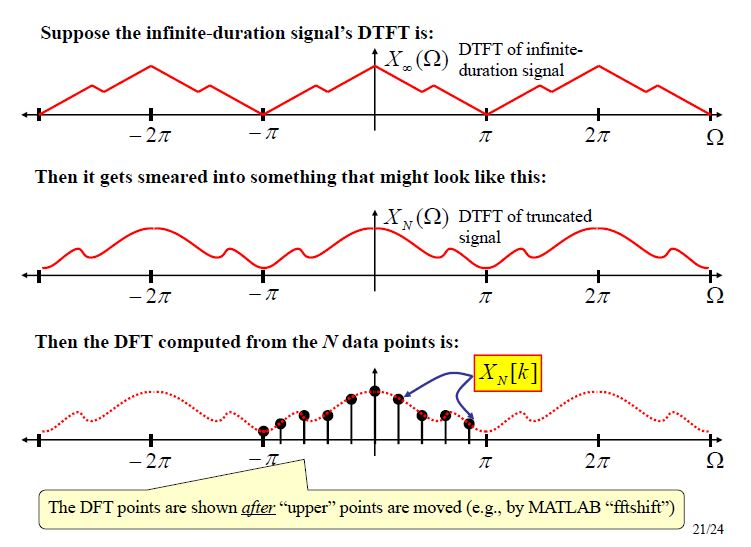
\includegraphics[width = 0.5\textwidth, frame]{Figures/DFT/what_DFT_give_us}
\caption{The DFT give us the smeared spectrum only}
\label{fig:DFT:what_DFT_give_us}
\end{figure} 



    \begin{itemize}
    
    \item The $\mathrm{2}^\mathrm{nd}$ is the smeared spectrum due to windowing 
    
    \item It is important to understand that the DFT will give us only the $\mathrm{2}^\mathrm{nd}$ row of \autoref{fig:DFT:what_DFT_give_us}
        
        \item In other words, truncation or windowing (source of error) cause a smeared spectrum (type of error)
        
        \item Another source of error is due to aliasing ( this is the $\mathrm{2}^\mathrm{nd}$ type of error we will explore its source later this later)
    \end{itemize}


    
\end{itemize}

\section{DFT for Spectral Analysis}

Now we move on for the practical use case of the DFT.

Say we have some signal we are interesting in analyzing its spectral content:

\begin{itemize}
    \item It could be a radar signal available only for a \tbi{short time}
    
    \item It could be some RF signal captured by an antenna, downcevert it and shifting it using a mixer then pass it through an ADC (or the ADC is near the antenna, and the ADC is in the bandpass mode)
\end{itemize}


\underline{\tbi{Design criteria}}: the real issue in DFT is when we reduce the samples we have for whatever the reason (signal available for only small time,$\cdots$) the resolution of the spectral component decrease.

So the big challenge is to do spectral analysis with high resolution with small amount of data.


\newpage
\subsection{Modeling the Truncation Problem}

\begin{figure}[h]
\centering
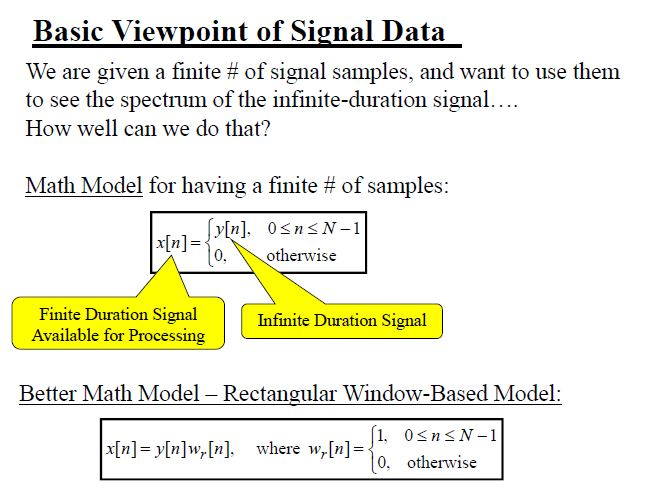
\includegraphics[width = 0.5\textwidth, frame]{Figures/DFT/truncation_modeling_1}
\caption{Truncation: using the rect window}
\label{fig:DFT:truncation_modeling_1}
\end{figure} 

\begin{itemize}
    
    \item We have some infinite signal $y[n]$ we can't collect it (recall from \autoref{Sec:DFT:Infinite_Duration} what are the other sources of infinity)
    
    \item The actual finite signal we have is $x[n]$
    
    \begin{itemize}
        \item A better mathematical modeling is the multiplication by the rect window
    \end{itemize}
    
    
    \item Be aware that in reality, all we do is collecting $N$ samples
    
    \begin{itemize}
        \item But to analyze this problem mathematically, we use the windowing idea: all the samples are given into some window and outside this window the values of these samples are 0
    \end{itemize}
    
\end{itemize}

The multiplication in time domain give us a convolution in the frequency domain, as shown in \autoref{fig:DFT:truncation_modeling_2}

\begin{figure}[h]
\centering
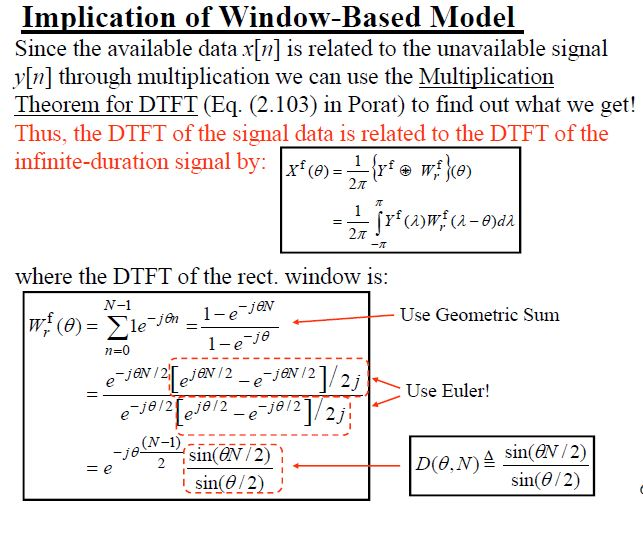
\includegraphics[width = 0.5\textwidth, frame]{Figures/DFT/truncation_modeling_2}
\caption{Truncation: using the rect window}
\label{fig:DFT:truncation_modeling_2}
\end{figure} 

\begin{itemize}
    \item The DTFT of a rect is not exactly a sinc function: it is a Drichlet function
\end{itemize}

In \autoref{fig:DFT:truncation_modeling_3}, we have the amplitude spectrum of the Drichlet for 2 values of $N$

\begin{figure}[h]
\centering
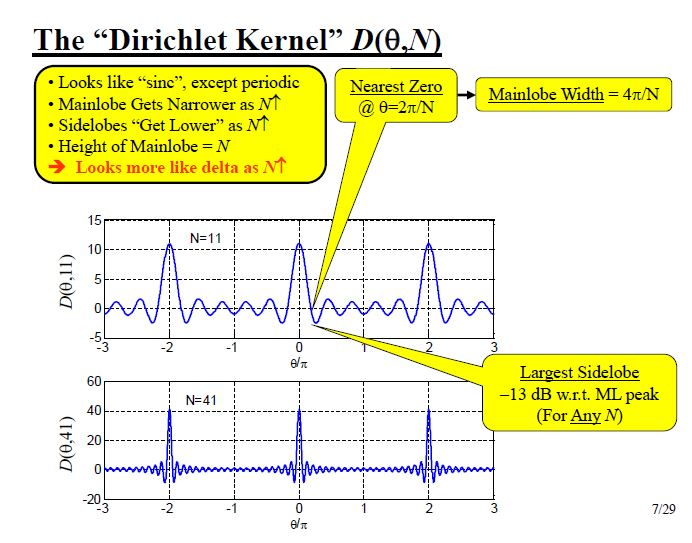
\includegraphics[width = 0.5\textwidth, frame]{Figures/DFT/truncation_modeling_3}
\caption{Truncation: using the rect window}
\label{fig:DFT:truncation_modeling_3}
\end{figure}

\begin{itemize}
    \item for a bigger $N$, 
    
    \begin{itemize}
    
        \item The mainlobe width get's smaller, converging into a delta $\leftrightarrow$ less leakage

        \item the maximum get's bigger
        
        \item But the side lobes won't get smaller 
    
    \end{itemize}
    
    
\end{itemize}


\autoref{fig:DFT:truncation_example_effect} show an example of the convolution example

\begin{figure}[h]
\centering
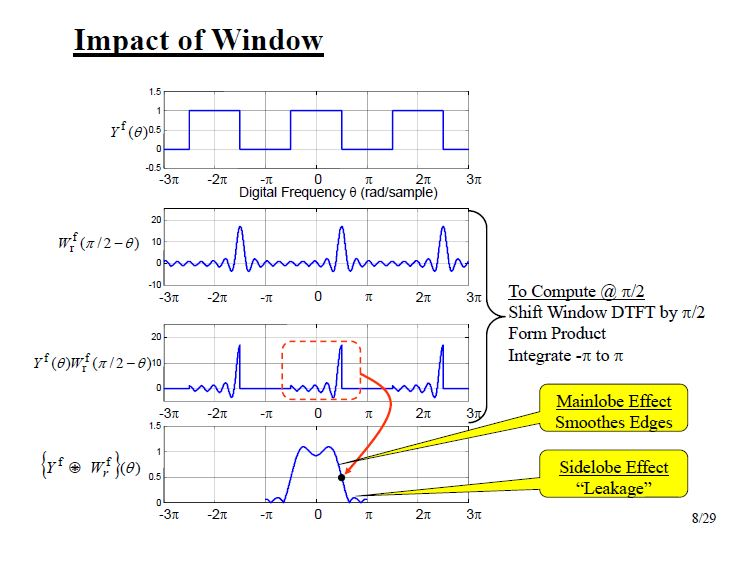
\includegraphics[width = 0.5\textwidth, frame]{Figures/DFT/truncation_example_effect}
\caption{Truncation: Exmaple}
\label{fig:DFT:truncation_example_effect}
\end{figure}

\begin{itemize}
    \item $Y(\theta)$ is the true DTFT
    
    
    \item In the $\mathrm{2}^\mathrm{row}$ we have the Drichlet shifted at $\displaystyle\frac{\pi}{2}$
    
    \item We do the multiplication and then do the intergral to obtain 1 value at the last line
    
    \item if we want to obtaine other values, we repeat the same process (sliding the window) for other values then $\displaystyle\frac{\pi}{2}$
    
    \item Notice that if the Drichlet main lobe was thinner (like a Dirac), the transition band would be sharper in the last row    
    
\end{itemize}


\section{Example}

This section take the causal exponential example, and try to simulate it to illustrate all the points we learned so far, which are summarized in \autoref{fig:DFT:Error_Types_DFT_Analysis} \\


\begin{figure}[h]
\centering
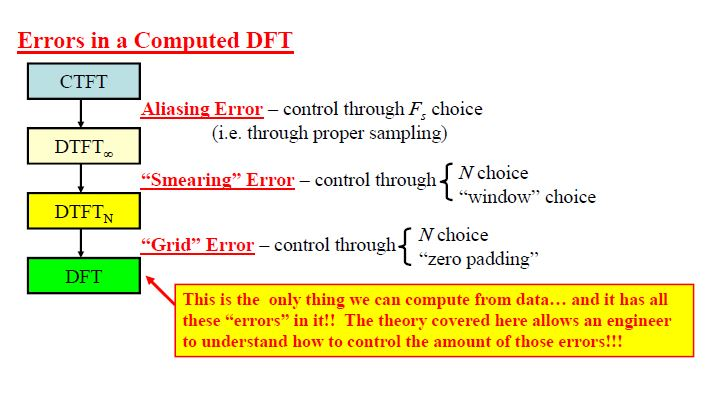
\includegraphics[width = 0.5\textwidth, frame]{Figures/DFT/Error_Types_DFT_Analysis}
\caption{Error Types in a DFT Analysis}
\label{fig:DFT:Error_Types_DFT_Analysis}
\end{figure}

Remember that in real world, all we can do is the DFT, and all the other things we can't do it since we don't necessarily have theoretical expression for the correspondent FT (CTFT or DTFT).


%******************************
%******************************
%******************************



\chapter{DFT V3}

\section{Introduction}

This chapter contains note about the DFT taken from chapter 3 in \cite{book_understanding_dsp}.


\section{Notes}

\begin{itemize}
    \item DFT Equation:
    
    
    \begin{equation}
        X[k] \, = \, \displaystyle\sum_{n \, = \, 0}^N x[n] \, \exp{\left(\, \displaystyle\frac{-j 2\pi \, n }{N} \, k \,\right)}
    \end{equation}
    
where: $\begin{cases}
k: \text{frequency index from } 0 \rightarrow N \, - \, 1 \\ 
x[n]: \text{input sequence of length }  N \\
n: \text{time domain index for the sequence } x[n]
\end{cases}$    
    
\item DFT compute the spectrum content of $N$ equally spaced frequency points    
    
\item $N$: is an important parameters since it determine 

\begin{enumerate}
    \item how much input samples are needed,
    
    \item  the resolution of the frequency domain result
    
    \item The amount of computation
\end{enumerate}
    
\item The frequency spacing: for a sampling rate $F_s$ and $N$ discrete time input sequence, the fundamental frequency in a DFT analysis is:

\begin{equation}
    \text{Fundamental Frequency} \, = \, \displaystyle\frac{F_s}{N}
    \label{Eq:DFTV3:Fundamental_Frequency}
\end{equation}

All the other frequencies will be multiple of \autoref{Eq:DFTV3:Fundamental_Frequency} $\leftrightarrow \, k \, \times \, \displaystyle\frac{F_s}{N}$.    
    
    
\newpage    
\item \underline{Leakage:}\\ 

To illustrate leakage, we give some example.

Suppose we have the following time domain signal:

\begin{equation}
x(t) \, = \, \sin{\left( \, 2 \pi 1000 \, t\,\right)} \, + \, 0.5 \, \cos{\left(\, 2 \pi 2000 \,t \, + \, \displaystyle\frac{\pi}{4}\,\right)}      
\end{equation}

If we take $N \, = \, 8$ and $F_s \, =\, 8000$ Hz, then the frequencies produced by DFT analysis (using $k \, \times \, \displaystyle\frac{F_s}{N}$):$0 \, , \, 1000\, ,\, 2000 , \, \cdots$.

Notice that the frequency bins produced by \autoref{Eq:DFTV3:Fundamental_Frequency} coincide with the  frequencies of $x(t)$. However, in real word signals we can't control usually this choice. This phenomena is what we call \tbi{leakage}.\\

Leakage can be reduced, but can't be eliminated , so we will try to understand it more.\\

The leakage problem is also treated from another starting points in different references:

\begin{itemize}
    \item For example chapter 7 in \cite{DSP_DimitrisManolakis}, they introduce the leakage through the windowing problem, and not directly manipulating the DFT equation
    
    
    \item Also they provide a good examples to illustrate what happens if the DFT bins doesn't coincide with input signal frequency
    
    
    \item The best window to use to minimize the effect of leakage and also provide a tradeoff between leakage and resolution is the Hann window
    
    
\end{itemize}

\todo{Leakage:} to do this in simulation later and \tbi{unify all these concepts}.



    
\end{itemize}








%******************************
%******************************
%******************************



\chapter{Windowing}

\underline{Source:} 

\begin{itemize}

    \item See chapter 6 in \cite{book_a_course_in_DSP_Porat}

    \item See lecture note \textit{Windows for Spectral Analysis of Signals 23} for figures and reference.
\end{itemize}



\section{Design Criteria of a Window}

\begin{itemize}

\item \underline{Slide 3}: focus on the design of window and what we need as characteristics in some particular window

\begin{itemize}
    \item Low side lobes and a rapid rate of decay
    
    \item Narrow main lobe
    
    
    \item Always a tradeoff between these 2
    
\end{itemize}


\item \underline{Slide 4}: The rectangular window has the narrowest main lobe among all the windows we will see

\begin{itemize}
    \item Side-lobe drop off rate: -6 dB/octave: octave is the double of the frequency.
    
    At each double frequency point, the side-lobe magnitude in dB decrease by 6.\\
    
    But around $\pm \pi$, the side-lobes remain constant

    
\end{itemize}

\end{itemize}


\section{Window Comparison}

\begin{itemize}

\item \underline{Slide 5-6}: Barlette Window (known also as triangular)

\begin{itemize}
    \item The idea is to lower the side-lobes level
    
    
    \item So he squared the magnitude of a rect window in frequency domain $\leftrightarrow$ convolution of 2 rect window in the time domain of size $\displaystyle\frac{N}{2}$ per window (to obtain a window of size $N$)
    
    \item As a result of this squaring, the side lobe ratio $ \left( \, \displaystyle\frac{\text{Main lobe amp}}{\text{side lobe amp}} \, \right)$ compared to a rect window has decreased
    
    
    \item Barlett has a continuity near the edge of the window (the continuity will have influence on the rate of decay of the side lobe levels)
    
    
    \item But the cost is a higher main lobe
    
\end{itemize}

\item \underline{Slide 7-8}: Hann window

\begin{itemize}
    \item He did a shifting in the frequency of rectangular window to cancell as much as he can the side lobe
    
    \item The largest side lobe level is bettet then Barlette: it is -32 dB vs -27 dB for Barlette
    
    \item And has a faster rate of decay for the side lobes compared to Barlette
    
    
\end{itemize}


\item \underline{Slide 9-10}: Hamming window

    \begin{itemize}
        \item Hamming took the idea of Hann and play on the amplitude factor
        
        \item He succeeded to obtain a lower side lobe level compared to Hann (- 43 dB compared to -32 dB for Hann)
        
        \item But the decay rate of the side lobes are much slower (6 dB/octave): this is because of the discontinuity of  the Hamming at the edge of the window
        
    \end{itemize}


\end{itemize}


\section{Derivative,Continuity and Rate of Decay}

\todo{Rate of Decay} Rate of Decay and Derivative concept: to be revisited later to see how to take derivatives as examples.

For now, I will write the main ideas

\underline{Slide 11}

\begin{itemize}
    \item In this section, we think in window in continous time to be able to use the concept of derivative
    
    \item For a rect: if we integrate we obtain a triangular function which is continuous, so $p \, = \, 0$ in this case
    
        \begin{itemize}
            \item We can't do derivative because it will give 0 
            
            \item trinagular: it will give us some function if we take the derivative, so $p \, = \, 1$
        \end{itemize}
    
    
\end{itemize}